% File name: datalogger/3DAQ/Documentation/Data_Transmission_Setup.tex
% Description of how data and commands will be transmitted between board and pc.
% Author: adh
% Date: Fri 24 May 2013 16:17

\documentclass[a4paper,11pt]{article}  % Standard document class
\usepackage[english]{babel}            % Set document language
\usepackage{fullpage}                  % Set up page for small margins etc

\usepackage{graphicx}                  % For including images in document
\usepackage{placeins}                  % Allows use of \FloatBarrier
% to avoid images or tables
% moving into next section
\usepackage{subfig}                    % For subfigures...

\usepackage{amsmath}                   % For improving maths/formula typesetting
\usepackage{tabularx}                  % Table changing package

\usepackage{algpseudocode}             % For producing algorithms/flowcharts
\usepackage{listings}                  % For including source code in document


% Provide command for scientific notation
\providecommand{\e}[1]{\ensuremath{\times10^{#1}}}
\providecommand{\degrees}{\ensuremath{^{\circ}}}

% Define title here:
\title{Communication and Data Transfer Protocol}
\author{James Glandular\\ jg597 \and Andrew Holt\\ ah635}
\date{24 May 2013}

\begin{document}

% generate title
\maketitle

\noindent The data logger works in 2 modes:

\begin{description}
  \item[Streaming Mode:] board is linked to computer and data is
    streamed up to the computer directly.
  \item[Standalone Mode:] board is not connected and stores data in
    EEPROM. The data is later transferred to the computer.
\end{description}

\section{Streaming Mode}

\begin{itemize}
  \item Every period, the board will send a packet of data to the
    computer.
  \item Each packet is 10 bytes long.
  \item The first 2 bytes will contain temperature data, and the third
    byte will contain humidity data. The rest will contain
    accelerometer data but not yet specifically defined.
\end{itemize}

\begin{center}
  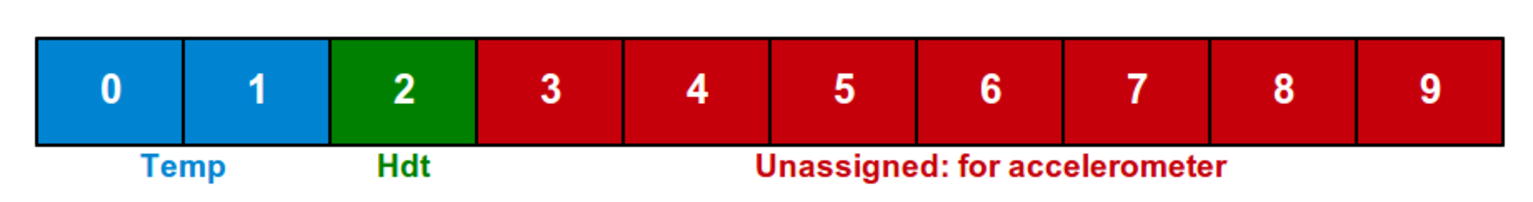
\includegraphics[width=0.8\textwidth]{Packet_diagram.pdf}
\end{center}

\section{Standalone Mode}

\begin{itemize}
  \item All collected data will be stored in the EEPROM, which
    contains 32,000 bytes.
  \item The first 16 bytes will contain configuration data.
  \item The first 2 of these will contain the length of the recorded
    data in bytes.
  \item The third will contain the sampling period, in seconds.
  \item The rest of the EEPROM will contain 10 byte packets, as in the
    streaming mode.
\end{itemize}

\section{PC to MCU Communication}

Commands will be sent by the PC software to the MCU for control of
logging in streaming mode and uploading and erasing data from the
EEPROM from standalone mode operation.
\begin{itemize}
\item All commands will be 10 bytes.
  \item When in streaming mode, \texttt{L} will be sent to begin
    logging and S will be sent to stop logging.
  \item When dealing with data from standalone operation, \texttt{U}
    will be sent to begin the upload process and \texttt{E} will be
    sent to erase the EEPROM memory (except the 16 configuration
    bytes)
  \item The sample rate may be set by sending \texttt{R} followed by
    the length of the desired sample period in seconds. For example,
    \texttt{R 128} will give a sample period of 128 seconds.
\end{itemize}

\end{document}